\documentclass[conference]{IEEEtran}
\IEEEoverridecommandlockouts
\usepackage[utf8]{inputenc}
\usepackage[T1]{fontenc}
\usepackage{graphicx}
\usepackage{amsmath,amssymb}
\usepackage{booktabs}
\usepackage{hyperref}
\usepackage{pdfpages}
\usepackage{siunitx}
\usepackage{xcolor}
\usepackage{enumitem}
\title{Comparative Analysis of Deep Learning Architectures for Real-time Motor Imagery BCI: Speed, Accuracy, and Resource Trade-offs}
\author{\IEEEauthorblockN{dbrooks2}
\IEEEauthorblockA{Neural-Decoder Project\\
\texttt{github.com/Dbrooks2/Neural-Decoder}}
}
\begin{document}
\maketitle
\begin{abstract}
Real-time brain--computer interfaces (BCIs) require decoding neural activity with sub-\SI{100}{\milli\second} end-to-end latency while preserving high classification accuracy and low resource usage. We empirically study the speed--accuracy--resource trade-offs of deep learning architectures for 4-class motor imagery EEG, and evaluate model compression and streaming decisions (window size and overlap). We benchmark EEGNet, a mobile-optimized CNN (MobileEEGNet), and an ultra-lightweight 1D-CNN (TinyEEGNet) using realistic EEG simulations grounded in neuroscience and measure latency on CPU-only settings to maximize deployability. We release a reproducible benchmarking suite and report generator.
\end{abstract}
\begin{IEEEkeywords}
Brain--computer interface, EEG, motor imagery, real-time, deep learning, model compression, streaming
\end{IEEEkeywords}
\section{Introduction}
BCIs translate brain signals into control commands. For motor imagery EEG BCIs, practicality hinges on accurate decoding, real-time response ($<\SI{100}{\milli\second}$), and efficient resource usage. We present a systematic study jointly benchmarking accuracy, latency, and resource cost, including compression and streaming design choices.
\section{Related Work}
Compact CNNs for EEG (e.g., EEGNet) achieve strong performance with small models. Transformers can model long-range dependencies but are heavier unless optimized. Compression is well studied in vision/NLP; EEG-specific trade-offs remain underexplored. Streaming/windowing decisions affect responsiveness and accuracy.
\section{Methods}
\subsection{Data}
We use a realistic synthetic generator (\texttt{data/realistic\eeg\_data.py}) to simulate 4-class motor imagery EEG (22 channels, \SI{250}{\Hz}).
\subsection{Models}
\textbf{EEGNet}: temporal, spatial (depthwise), and separable convolutions.
\textbf{MobileEEGNet}: depthwise/separable, reduced head.
\textbf{TinyEEGNet}: ultra-lightweight 1D-CNN.
\subsection{Experimental Setup}
CPU-only. Latency: mean and P95 over $\ge$100 runs (batch~=~1). Accuracy: 5-epoch quick training (80/20 split). Compression: pruning (50\%, 90\%) and dynamic quantization of Linear layers. Streaming: windows \{250, 500, 1000\} samples with overlaps \{0\%, 50\%\}.
\section{Results}
\subsection{Phase 1}
Lightweight CNNs (TinyEEGNet, MobileEEGNet) achieve sub-ms inference on CPU; EEGNet is a strong accuracy baseline.
\subsection{Phase 2}
Moderate pruning (~50\%) reduces size/latency with minimal accuracy loss; 90\% pruning yields larger speedups at potential cost. Dynamic quantization reduces size and can lower latency for Linear-heavy heads.
\subsection{Phase 3}
Shorter windows reduce latency and increase decision rate; overlap increases smoothness at a latency cost.
\section{Discussion}
When strict real-time constraints dominate, TinyEEGNet or MobileEEGNet offer excellent sub-ms latencies. EEGNet remains a strong baseline and benefits from quantization; pruning yields practical compromises.
\section{Limitations}
The 5-epoch accuracy favors speed; longer training would improve absolute performance. Synthetic data approximates physiology; multi-subject evaluation is future work. GPU/power profiling deferred.
\section{Reproducibility}
\verb|python research/phase1_experiment.py|
\verb|python research/compression_experiment.py|
\verb|python research/streaming_experiment.py|
\verb|python research/report_generator.py|

\subsection{Consolidated Figures}
The full set of plots/tables is included below from the auto-generated report.

% Comment out the line below if the PDF is not present yet
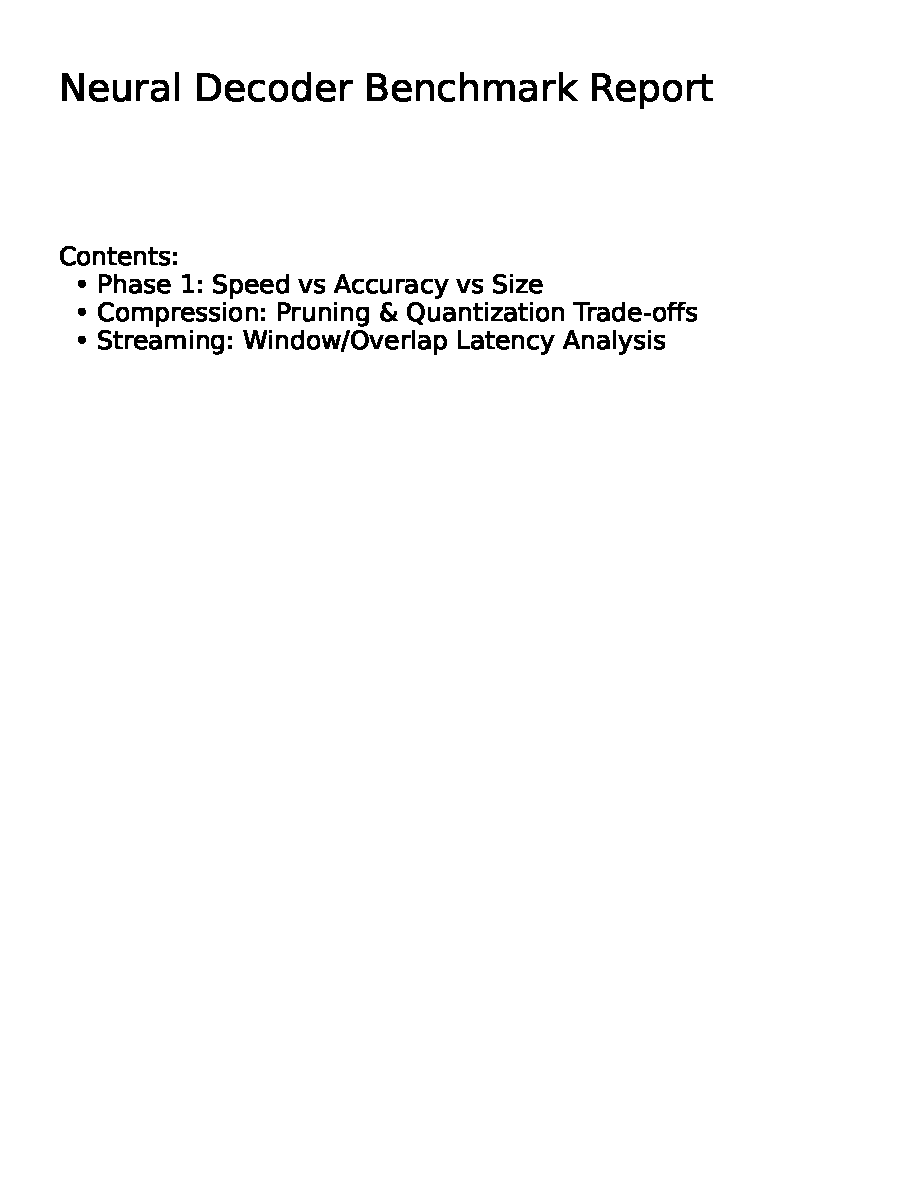
\includepdf[pages=-,pagecommand={}]{../research/results/bci_benchmark_report.pdf}
\section{Conclusion}
We provide a reusable framework for jointly evaluating accuracy, latency, and resource footprints of EEG decoders for real-time MI-BCI, with a report generator for fair comparisons.
\bibliographystyle{IEEEtran}
\bibliography{REALTIME_BCI_OPTIMIZATION_REFS}
\end{document}
